% TeX encoding = utf8
% TeX spellcheck = pl_PL 
\documentclass[a4paper, 11pt]{article}
\usepackage[utf8]{inputenc}
\usepackage[polish]{babel}
\usepackage{polski}
\usepackage{graphicx}
\usepackage{listings}
\usepackage{amsfonts}
\usepackage{geometry}
\usepackage{multicol}
\usepackage{latexsym}
\usepackage{enumerate}
\usepackage{hyperref}
\usepackage{color} %red, green, blue, yellow, cyan, magenta, black, white
\definecolor{mygreen}{RGB}{28,172,0} % color values Red, Green, Blue
\definecolor{mylilas}{RGB}{170,55,241}

\author{Kamil Foryszewski}
\title{Dokumentacja projektu laboratoryjnego numer 1 przedmiot MNUM}
\frenchspacing

\newgeometry{tmargin=2cm, bmargin=2cm, lmargin=2cm, rmargin=2cm}
\pagestyle{empty}


\begin{document}

\lstset{language=Matlab,%
    basicstyle=\color{red},
    breaklines=true,%
    morekeywords={matlab2tikz},
    keywordstyle=\color{blue},%
    morekeywords=[2]{1}, keywordstyle=[2]{\color{black}},
    identifierstyle=\color{black},%
    stringstyle=\color{mylilas},%
    commentstyle=\color{mygreen},%
    showstringspaces=false,
    numbers=right,%
    numberstyle={ \color{black}},% size of the numbers
    numbersep=5pt, % this defines how far the numbers are from the text
    emph=[1]{for,endfor,endwhile,endfunction,endif,break},emphstyle=[1]\color{blue}, %some words to emphasise
    emph=[2]{,.}, emphstyle=[2]\color{yellow},%
}

\maketitle
\tableofcontents


\section{Epsilon maszynowy}

\subsection{Polecenie}
Proszę napisać program wyznaczjący dokładność maszynową komputera i wyznaczyć ją na swoim komputerze.
\vspace{0,5cm}

\subsection{Opis teoretyczny}
\indent

Epsilon maszynowy jest to maksymalny błąd względny reprezentacji zmiennoprzecinkowej. Zależy on jedynie od liczby bitów mantysy i nazywany jest dokładnością maszynową.~\cite{first} Aby go wyznaczyć należy znaleźć najmniejszą nieujemną liczbę, która dodada do jedności daje wynik różny od jedności. Nie należy mylić go z dużo mniejszą liczbą nazywaną liczbą róźną od zera, którą wyznacza się w podobny sposób. Epsylon maszynowy jest zależny od liczby bitów mantysy w reprezentacji zmiennoprzecinkowej. Epsilon maszynowy możemy wyznaczyć przy pomocy następującego algorytmu podanego jako lista kroków:
\begin{enumerate}
  \item $a = 1, b = 2$
  \item dopóki $a$ różne od $1$ $eps = x/2, b = 1 + x$
  \item wyświetl eps
\end{enumerate} 
Poniżej kod programu wyznaczającego epsilon maszynowy w programie Matlab:


\subsection{Realizacja w programie Matlab}

\begin{lstlisting}
% Obliczanie epsilona maszynowego 
  a=1.0; %wartosci poczatkowe
  b=2.0; 
 
% Epsilon maszynowy 
  while( b != 1)
      epsilon=a; 
      a=a/2; 
      b=1.0+a; 
  end
  
  printf('Obliczona wartosc epsilon:\n')
  disp(epsilon)
  printf('Stala epsilon zaimplementowana w Matlabie:\n')
  disp(eps)
  
  
% Najmniejsza liczba rozna od 0
  a = 1.0;
  while(a != 0)
    dbl_eps = a; 
    a = a/3; 
  end
  printf('Obliczona najmniejsza liczba rozna od 0:\n')
  disp(dbl_eps)

\end{lstlisting}

\vspace{1cm}

\subsection{Wynik działania programu}

Obliczona wartość epsilon:\\
	2.2204e-16\\
Stala epsilon zaimplementowana w Matlabie:\\
	2.2204e-16\\
Obliczona najmniejsza liczba róźna od 0:\\
	4.9407e-324\\
	
\subsection{Wnioski}
\indent 

Obliczony epsilon maszynowy jest równy stałej eps występującej w środowisku Matlab, liczba ta jest zgodna z wielkością epsylon dla liczb podwójnej prezyzji w reprezentacji 64-bitowej według standardu IEEE 754. 
Ponadto obliczony epsilon jest rzędy wielkości większy od obliczonej najmniejszej liczby rożnej od 0. Dlatego nie należy mylić tych pojęć.~\cite{second}


\section{Metoda elminacji Gaussa z częściowym wyborem elementu głównego}

\subsection{Polecenie}
Proszę napisać program rozwiązujący układ $n$ równań liniowych $Ax = b$ wykorzystując metodę eliminacji Gaussa z częściowym wyborem elementu głównego. Proszę zastosować program do rozwiązania podanych niżej układów równań dla rosnącej liczby równań $n = 10, 20, 40, 80, 160$ \dots Liczbę tych równań proszę zwiększać aż do momentu, gdy czas potrzebny na rozwiązanie układu staje się zbyt duży (lub metoda zawodzi).

\subsection{Opis teoretyczny}
Metoda eliminacji Gaussa należy do metod skończonych, to znaczy że wynik otrzymujemy po określonej skończonej liczbie operacji zależnej od wymiarowości zadania. Aby wyznaczyć rozwiązanie równania mazieżowego $Ax = b$ należy w pierwszej kolejności przeprowadzić eliminację zmniennych. Metoda ta prowadzi do powstania mazieży trókątnej, na podstawie której wyznaczamy wartości poszczególnych składowych wektora rozwiązań, poprzez metodę postępowania odwrotnego.~\cite{third}

\subsubsection{Metoda LU}
Metoda polega na przekształceniu wyjściowej macierzy $A$ do postaci iloczynu macierzy $PA = LU$ gdzie $P$ - macierz permutacji związana z wyborem elementu głównego, $L$ - macierz trójkątna dolna z jedynkami na diagonali oraz $U$ - macierz trójkątna górna. Zakładamy że rozkład $A = LU$ istnieje. Wtedy prawdzie jest równanie z wyeksponowanym pierwszym wierszem i kolumną:

$$
\left( \begin{array}{ccc}
a_{11}^T & a_{12} \\
a_{21} & A_{22} \\
\end{array} \right)
=
\left( \begin{array}{ccc}
1 & 0^T \\
l_{21} & L_{22} \\
\end{array} \right)
\left( \begin{array}{ccc}
u_{11} & u_{12}^T \\
0 & U	_{22} \\
\end{array} \right)
$$

Teraz mnożąc blokowo macierz $L$ przez $U$ :
\begin{itemize}
\item $u_{11} = a_{11}$ oraz $u_{12} = a_{12} \to $ pierwszy wiersz $U$ jest kopią pierwszego wiersza $A$
\item $l_{21} = a_{21}/u_{11} \to$ pierwsza kolumna $L$ powstaje przez podzielenie wektora $a_{2:}$ przez element na diagonali.
\item $A_{22} - l_{21}u_{12}^T = L_{22}U_{22} \to$ znalezienie podmacierzy $L_{22} , U_{22}$ sprowadza się do znalezienia rozkładu $LU$ zmodyfikowanego bloku $A_{22}$ macierzy $A$ o wymiarze $(n-1)\times(n-1)$. Procedurę tą nazywamy uzupełnieniem Schura.
\end{itemize}

Jest to algorytm rekurencyjny, który można zastąpić pętlą, oszczędzając przy tym pamięć i czas. Algorytm będzie wykonywany w miejscu tzn. elementy macierzy $L,U$ będą zapisywane w miejscach elementów macierzy $A$. Pamiętając o jedynkach na diagoinali.\\


\textbf{Wybór elementu głównego}\\
\\
Aby zapobiec sutuacji dzielenia przez zero, dokonujemy kolumnowego wyboru elementu głównego realizując następujące kroki:
\begin{itemize}
\item w pierwszej kolumnie podmacierzy $A(k:n,k:n)$ szukamy elementu o największym module. 
\item zamieniamy wiersze $A(k,1:n)$ z wierszem zawierającym element główny.
\item zapamiętujemy permutację poprzez wpisanie do (początkowo jednostkowej) macierzy $P$ jedynek w miejscach przecięcia numerów zmienionyh wierszy. Późniejsze pomożenie przez macierz $P$ powoduje zamianę wierszy identyczną jak przy powyższym algorytmie.~\cite{fourth}
\end{itemize}

\textbf{Złożoność obliczniowa}\\
\\
Jak wynika z przedstawionego algorytmu $k$-ty obrót pętli wymaga $2(n-k)^2$ operacji. Stąd łączny koszt rozkładu wynosi w przybliżeniu $\frac{4}{3}n^3$.\\

\textbf{Realizacja w programie Matlab}\\
\\
W celu późniejszego wykorzystania metody została ona zaimplementowana jako funcja zwracająca macierz $LU$ oraz macierz permutacji $P$ dla argumentu $A$.

\begin{lstlisting}
% funkcja zwracajaca podzial LU macierzy kwadratowej
function [LU,P] = lucw (A)

  n = size(A)(1,1);
  
  if n!=size(A)(1,2) 
    print('macierz nie jest kwadratowa');
  endif
  P = eye(n); %macierz transformacji
  LU = A; 
  
  for k = 1:n-1
      
    [void pos] = max(abs(LU(k:n,k))); %wybor elementu glownego
    pos=pos+k-1;
  
    if(pos~=k) % zamiana wierszy
      temp = LU(pos,:);
      LU(pos,:) = LU(k,:);
      LU(k,:) = temp;
        
      P(k,k) = 0; % zapis zmiany wierszy do macierzy transformacji
      P(pos,pos) = 0;
      P(k,pos) = 1;
      P(pos,k) = 1;
    end
             
    for i = k+1:n % normalizacja podmacierzy pod elementem glownym
          
      LU(i,k) = LU(i,k)/LU(k,k); %wyznaczanie k-tej kolumny
      LU(i,(k+1):n) = LU(i,(k+1):n) - LU(i,k)*LU(k,(k+1):n);
      
    end
    
  end
  
end

\end{lstlisting}

\subsubsection{Rozwiązanie układu z macierzą trójkątną}

Powstały rozkład $LU$ zostanie wykorzystany do obliczenia wartości wektora rozwiązań $x$. 
Aby wyznaczyć rozwiązanie układu należy:
\begin{itemize}
\item Obliczyć w pierwszej kolejności $Ly = b$ 
\item Następnie powstałego wektora $y$ użyć do rozwiązania równania $Ux = y$
\end{itemize}
W pierwszym przypadku należy rozwiązać równanie z macierzą trójkątną dolną. Jest to proste zadanie w którym wyznaczamy elementy wektora wynikowego kolejno. $x_i = b_i\,-\,\sum_{j=1}^{i-1} l_{i,j} x_j^*$
układ z macierzą trójkątną górną rozwiązujemy metodą podstawiania w tył. $x_i^*\,:=\,\left( b_i\,-\, \sum_{j=i+1}^n u_{i,j}x_j^*\right)/u_{i,i}$\\

\textbf{Złożoność obliczniowa}\\
\\
Złożoność obliczeniowa przy rozwiązywnaiu układu z macierzą trójkątną wynosi $n^2$.\\

\textbf{Realizacja w programie Matlab}\\
\\
W celu późniejszego wykorzystania metody została ona zaimplementowana jako funkcja zwracająca wektor rozwiązań $x$ dla argumentów $LU,P,b$.

\begin{lstlisting}
% funkcja wyznaczjaca rozwiazania ukladu dla macierzy LU
function [x] = lufx (LU,P,b)

  n = size(b)(1,1); % zbadanie wymiaru macierzy

  b = (P')*b; % pomnozenie wektora b przez transformowana macierz P

  %macierz trojkatna dolna Ly = Pb

  y(1,1) = b(1,1);

  for i = 2:n

    s = b(i,1);
  
    for j = 1:i-1
      s = s - LU(i,j)*y(j,1);
    end
  
    y(i,1) = s;
  
  end

  %macierz trojkatna gorna Ux = y

  x(n,1) = y(n,1)/LU(n,n);

  for i = n-1:-1:1

   p = y(i,1);
  
    for j = i+1:n
      p = p - LU(i,j)*x(j,1);
    end
  
    x(i,1) = p/LU(i,i);
  
  end

end

\end{lstlisting}

\subsection{Generowanie danych do obliczeń}
Dane do obliczeń zostały wygenerowane przez funkcję której argumentami są: ilość równań oraz podpunkt od 1 do 3 według polecenia:

$$
1) \ a_{ij} = \left\{ \begin{array}{ll}
10 & \textrm{dla $i=j$,}\\
5 & \textrm{dla $i=j-1$ lub $i=j+1$, \hspace{1cm} $b_{i} = 2+0,3i$;}\\
0 & \textrm{dla pozostalych,}
\end{array} \right.
$$
\hspace{3cm} $2) \ a_{ij} = 2(i-j)+1$ \hspace{1cm} $a_{ii} = \frac{1}{6}$ \hspace{1cm} $b_{i} =1+0,4*i$; \\

\hspace{2,4cm} $2) \ a_{ij} = \frac{8}{9(i+j+1)}$  \hspace{1cm} $b_{i} =\frac{4}{3i}$ $i$ parzyste; $b_{i} = 0$ $i$ - nieparzyste; \\

\vspace{1cm}

\textbf{Realizacja w programie Matlab}\\
\\
\begin{lstlisting}
%funkcja generujaca macierz 
function [A,B] = create_matrix (n,p)

  if (p==1)
   for i = 1:n
     for j = 1:n
       if (i==j)
         A(i,j) = 10;
       end
       if (i==j-1)
         A(i,j) = 5;
       end
       if (i==j+1)
         A(i,j) = 5;
       end
     end
     B(i,1) = 2 + 0.3*i;
   end
  end

  if (p==2) 
  for i = 1:n
    for j = 1:n
      if (i==j)
        A(i,j) = 1/6;
      else
        A(i,j) = 2*(i-j) + 1;
      end
    end
    B(i,1) = 1 + 0.4*i;
   end
  end

  if (p==3)
  for i = 1:n
    for j = 1:n
      A(i,j) = 8/(9*(i + j + 1));
    end
    if (mod(i, 2) == 0)
      B(i,1) = 4/(3*i);
    else
      B(i,1) = 0;
    end
   end
  end
  
end
\end{lstlisting}

\subsection{Wyniki działania programu}
W celu prezentacji wyników działania programu został napisany skrypt, wykorzystujący wcześniej utworzone funkcje do obliczenia błędów rozwiązań dla rozsnącej liczby równań, dla każdego zestawu danych z zadania. \\
\vspace{1cm}

\textbf{Realizacja w programie Matlab}\\
\\
\begin{lstlisting}
%Skrypt generujacy wyniki oraz wykresy
clear

F = fopen('results.txt','w'); %wynik zapisany do pliku

for i= 1:3 % iteracja po podpunktach

  for j= 0:7 % iteracja po liczbie rownan
  
  result(1,j+1) = 10*2^j; % zapamietanie liczby rownan
  
  t = cputime; % poczatek liczenia czasu

  [A,b] = create_matrix(10*2^j,i); % utworznie macierzy

  [LU,P] = lucw(A); % wyznaczenie rozkladu
  
  x = lufx(LU,P,b); % obliczenie wektora rozwiazan
  
  res = A*x - b;
  error = norm(res,1); % blad jako norma residuum
  
  result(2,j+1) = error; % zapamietanie bledu dla liczby rownan
    
  time = cputime-t; % obliczenie czasu wykonania
  
  fprintf(F, 'Podpunkt: %d ,Liczba rownan: %d , Blad: %g , Czas: %d sek. \n',i,result(1,j+1),result(2,j+1),time);

  end
  
  a = stem(result(1,:),result(2,:),'o','filled'); % utworzenie wykresu
  
  if(i==1)
    title('Plot 1');
    xlabel('number of eqations');
    ylabel('error');
    saveas(a, 'wykres1.png');
  
  elseif (i==2) 
    title('Plot 2');
    xlabel('number of eqations');
    ylabel('error');
    saveas(a, 'wykres2.png');
  else
    title('Plot 3');
    xlabel('number of eqations');
    ylabel('error');
    saveas(a, 'wykres3.png');
  end
 

end

fclose(F);
\end{lstlisting}


\vspace{1cm}
\textbf{Zestaw danych 1}\\
\\

\textbf{Wynik działania programu:}\\
Podpunkt: 1 ,Liczba rownan: 10 , Blad: 2.22045e-15 , Czas: 0.023333 sek. \\
Podpunkt: 1 ,Liczba rownan: 20 , Blad: 3.9968e-15 , Czas: 0.04 sek. \\
Podpunkt: 1 ,Liczba rownan: 40 , Blad: 8.88178e-15 , Czas: 0.103334 sek. \\
Podpunkt: 1 ,Liczba rownan: 80 , Blad: 4.52971e-14 , Czas: 0.273333 sek. \\
Podpunkt: 1 ,Liczba rownan: 160 , Blad: 1.63425e-13 , Czas: 1.08 sek. \\
Podpunkt: 1 ,Liczba rownan: 320 , Blad: 6.21281e-13 , Czas: 4.36667 sek. \\
Podpunkt: 1 ,Liczba rownan: 640 , Blad: 3.0731e-12 , Czas: 18.1633 sek. \\
Podpunkt: 1 ,Liczba rownan: 1280 , Blad: 1.13651e-11 , Czas: 77.0833 sek.\\
\\
\vspace{11cm}
\textbf{Wykres zależności błędu od liczby równań}\\
\begin{figure}[th]
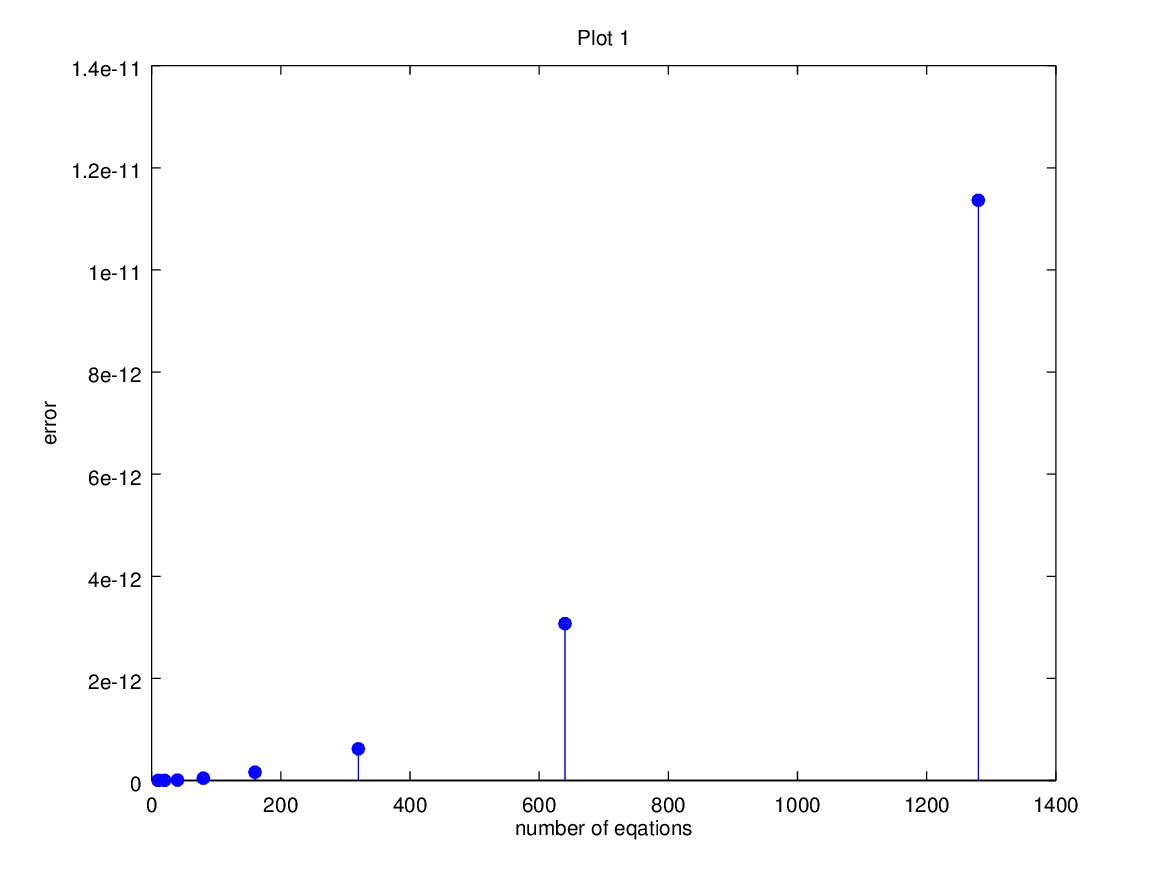
\includegraphics[width=\textwidth]{wykres1}
\end{figure}

\vspace{2cm}
\textbf{Wnioski}\\
\\
Dla pierwszego zestawu danych błąd rozwiązania jest stosunkowo niewielki i rośnie wraz z liczbą równań. 
Dla tego zadania macierz $A$ jest dobrze uwarunkowana, ponieważ jest diagonalnie silnie dominująca. Dla liczby równań powyżej 1280 czas potrzebny na  rozwiąznie staje się zbyt długi. 

\vspace{1cm}
\textbf{Zestaw danych 2}\\
\\

\textbf{Wynik działania programu:} \\
Podpunkt: 2 ,Liczba rownan: 10 , Blad: 30 , Czas: 0.006667 sek. \\
Podpunkt: 2 ,Liczba rownan: 20 , Blad: 135 , Czas: 0.033333 sek. \\
Podpunkt: 2 ,Liczba rownan: 40 , Blad: 578 , Czas: 0.193334 sek. \\
Podpunkt: 2 ,Liczba rownan: 80 , Blad: 2376 , Czas: 0.703333 sek. \\
Podpunkt: 2 ,Liczba rownan: 160 , Blad: 9750 , Czas: 1.19 sek. \\
Podpunkt: 2 ,Liczba rownan: 320 , Blad: 39732 , Czas: 4.81333 sek. \\
Podpunkt: 2 ,Liczba rownan: 640 , Blad: 160625 , Czas: 19.8533 sek. \\
Podpunkt: 2 ,Liczba rownan: 1280 , Blad: 646893 , Czas: 86.6033 sek. \\
\\
\vspace{1cm}
\textbf{Wykres zależności błędu od liczby równań}\\
\begin{figure}[th]
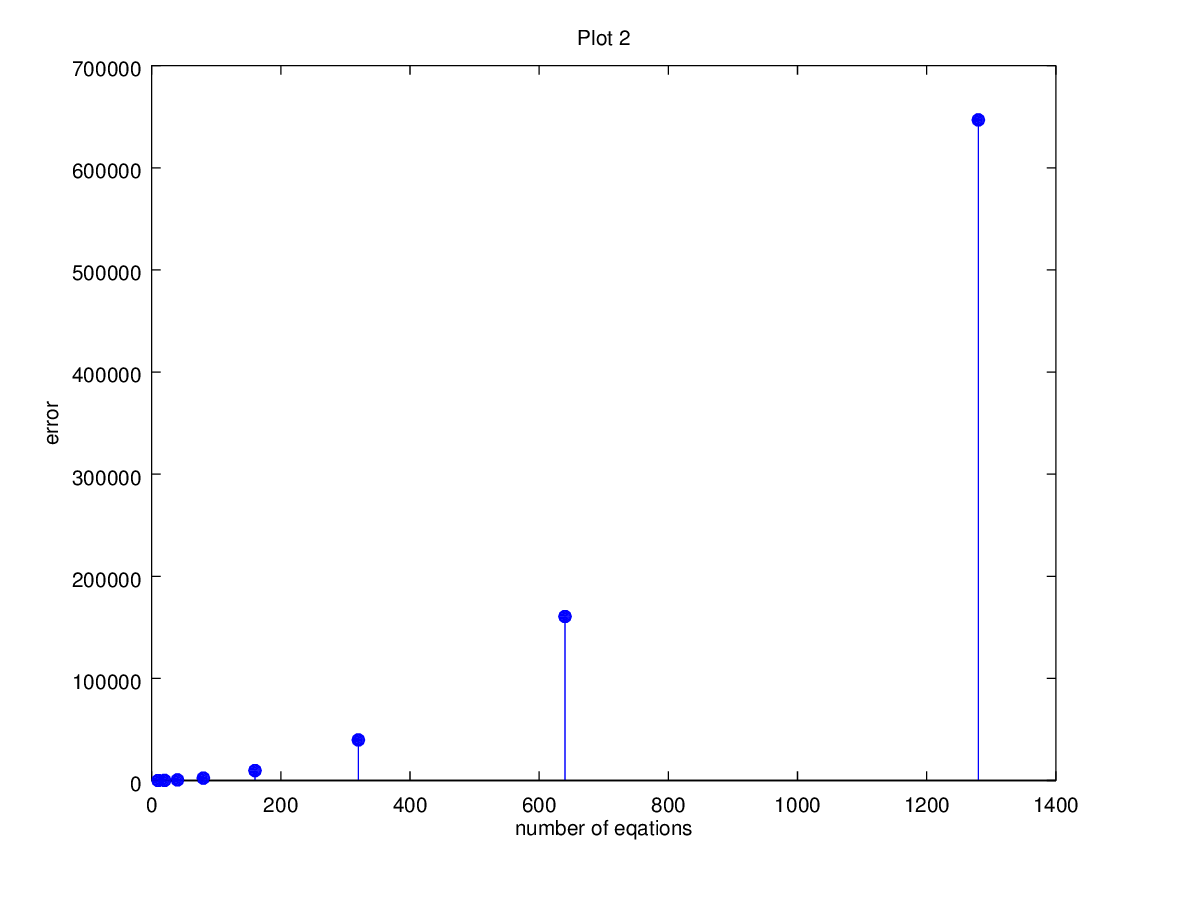
\includegraphics[width=\textwidth]{wykres2}
\end{figure}


\textbf{Wnioski}\\
\\
Dla drugiego zestawu danych błąd rozwiązania jest znacznie większy i rośnie wraz z liczbą równań. 
Elementy na diagonali są znacznie mniejsze co do modułu od pozostałych. Powoduje to pojawianie się wartości bliskich zeru podczas generowania macierzy $LU$, co prowadzi do dużych błędów w obliczeniach. Dla liczby równań powyżej 1280 czas potrzebny na rozwiąznie staje się zabyt długi. 


\vspace{1cm}
\textbf{Zestaw danych 3}\\
\\

\textbf{Wynik działania programu:} \\
Podpunkt: 3 ,Liczba rownan: 10 , Blad: 0.267628 , Czas: 0.01 sek. \\
Podpunkt: 3 ,Liczba rownan: 20 , Blad: 6.71819 , Czas: 0.046666 sek. \\
Podpunkt: 3 ,Liczba rownan: 40 , Blad: 29.2936 , Czas: 0.113333 sek. \\
Podpunkt: 3 ,Liczba rownan: 80 , Blad: 137.833 , Czas: 0.316667 sek. \\
Podpunkt: 3 ,Liczba rownan: 160 , Blad: 3683.93 , Czas: 1.15333 sek. \\
Podpunkt: 3 ,Liczba rownan: 320 , Blad: 826 , Czas: 4.68667 sek. \\
Podpunkt: 3 ,Liczba rownan: 640 , Blad: 294.727 , Czas: 19.2033 sek.\\ 
Podpunkt: 3 ,Liczba rownan: 1280 , Blad: 698.679 , Czas: 82.4 sek. \\


\vspace{1cm}
\textbf{Wykres zależności błędu od liczby równań}\\
\begin{figure}[th]
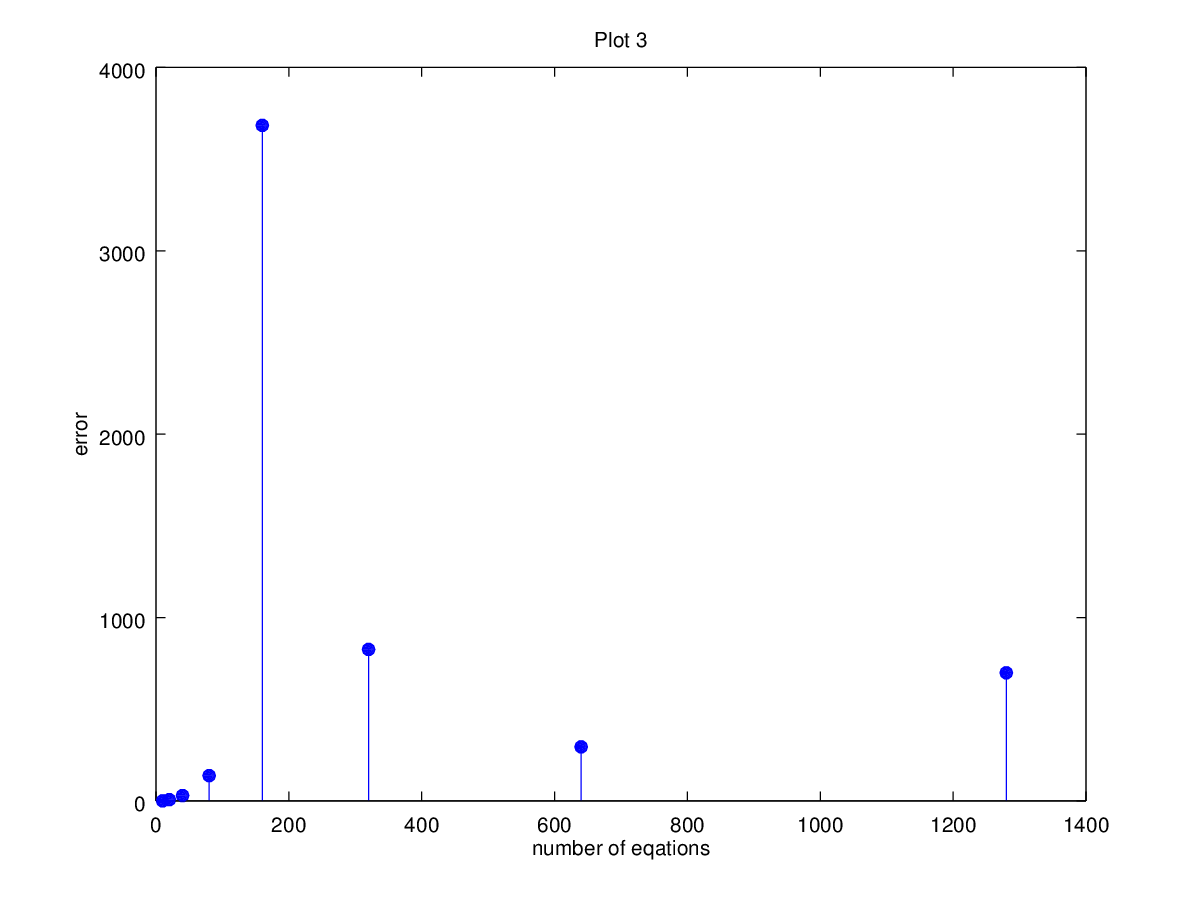
\includegraphics[width=\textwidth]{wykres3}
\end{figure}

\vspace{1cm}
\textbf{Wnioski}\\
\\
Dla trzeciego zestawu danych błąd rozwiązania jest duży, jednak nie można zdefiniować zeleżności pomiędzy nim a liczbą równań. Elementy macierzy $A$ są na tyle małe że podczas obliczeń przetwarzane są liczby w granicach dokładności obliczeniowej. Promień spektralny macierzy jest jednak niewieli dlatego błędy obliczeniowe nie są tak wysokie jak w przypadku podpunktu 2. Dla liczby równań powyżej 1280 czas potrzebny na rozwiąznie staje się zabyt długi.

\subsection{Poprawianie iteracyjne}
Dla liczby równań 10 zostało przeprowadzone iteracyjne poprawianie rozwiązań. Polega ono na wyznaczeniu \textsl{residuum} czyli błędu rozwiązania według wzoru $r = Ax -b$. Dzięki temu możemy wyznaczyć jaka zmiana $\delta x$ generuje nasz błąd. ~\cite{fifth}
Poprawienia dokładności rozwiązania możemy dokonać postępując następująco: 
\begin{itemize}
\item Wyznaczamy resztę $r = Ax -b$.
\item Rozwiązujemy układ $A\delta x = r$
\item Wyznaczamy nowy wektor rozwiązań $x^{(2)} = x^{(1)} -\delta x$.
\item Obliczamy kolejny raz resztę tym razem dla nowego $x$ i sprawdzamy czy spełnia założenia dokładności.
\end{itemize}

\textbf{Realizacja w programie Matlab}\\
\\
\begin{lstlisting}
% Funkcja realizujaca iteracyjne poprawianie
function [x] = grow (A,x,b,LU,P)

  r = A*x-b; % obliczenie reszty
  while (norm(r)>2*eps) % wykonuj jezeli blad wiekszy od 2eps
    o = r; 
    r = A*x-b;
    if(norm(r)<norm(o)) % jezeli blad rosnie zakoncz
      break; 
    end
    dx = lufx(LU,P,r); % obliczenie delta x
    x = x-dx; odjecie od wektora delta x
  end

end

\end{lstlisting}

\begin{lstlisting}

% Sktypt wyznaczajacy blad po poprawianu iteracyjnym
clear;

for i= 1:3 % iteracja po podpunktach
  
  [A,b] = create_matrix(10,i);

  [LU,P] = lucw(A);
  
  x = lufx(LU,P,b);
  
  res = A*x - b;
  error = norm(res,1); 
  
  printf('Blad dla zestawu: %d przed: %g,',i,error); 
   
  res1 = A*grow(A,x,b,LU,P) - b;% Poprawianie
  error1 = norm(res1,1);
  
  printf('Blad dla zestawu: %d po poprawianiu: %g,\n',i,error1);
  
end

\end{lstlisting}

\vspace{1cm}
\textbf{Wyniki działania programu}\\
\\
Blad dla zestawu: 1 przed: 2.22045e-15,Blad dla zestawu: 1 po poprawianiu: 1.33227e-15,\\
Blad dla zestawu: 2 przed: 30,Blad dla zestawu: 2 po poprawianiu: 23.2,\\
Blad dla zestawu: 3 przed: 0.267628,Blad dla zestawu: 3 po poprawianiu: NaN,\\

\vspace{2cm}
\textbf{Wnioski}\\
\\
Pętla iteracyjnego poprawiania wykonywała się do czasu wystąpienia dokładności rzędu $2eps$ lub do czasu kiedy błąd przestał maleć. Dla zestawów 1 i 2, iteracyjne poprawianie dało dokładniejszy wynik. Natomiast dla zestawu 3 metoda iteracyjnego poprawiania zawiodła. Stało się tak ponieważ wektor rozwiązań stanowiły liczby naprzemieie dodatnie i ujemne. Norma tego wektora była coraz mniejsza dlatego algorytm postępował dalej. Po wielu krokach iteracji wartości wektora rozwiązań zaczęły przekraczać zakresy reprezentacji liczb, stąd wynik NaN. 

\section{Metoda Jacobiego}
\subsection{Polecenie}
\indent

Proszę napisać program rozwiązujący $n$ równań liniowych $Ax=b$ wykorzystując metodę Jacobiego i użyć go do rozwiązania danego układu równań liniowych:\\
\\
$14x_{1}-x_{2} -3x_{3}+5x_{4} = 1$\\
$x_{1}-7x_{2} -4x_{3}-x_{4} = 0$\\
$2x_{1}-4x_{2} -12x_{3}-x_{4} =-10$\\
$x_{1}-x_{2}+6x_{3}-16x_{4} = -2$\\
\\
Proszę sprawdzić dokładność rozwiązania oraz spróbować zastosować zaprogramowaną metodę do rozwiązania układów równań z zadania 2. 

\subsection{Opis teoretyczny}
\indent

Metoda Jacobiego jest metodą iteracyjną. Oznacza to że aby uzyskać wynik należy wykonywać powtarzające się operacje na macierzy wyjściowej do momentu spełnienia założeń o wyniku działania. Aby rozwiązać układ równań $Ax=b$ należy dokonać dekompozycji macierzy $A = L+D+U$ gdzie macierz $L$ jest macierzą złożoną z elementów macierzy $A$ znajdującymi się pod diagonalą, macierz $D$ to macierz diagonalna skłądająca się z diagonali macierzy $A$ natomiast macierz $U$ składa się z elementów nad diagonalą $A$. \\
Układ $Ax=b$ można zapisać w postaci\\

\hspace{1cm} $Dx = -(L+U)x +b$ \\

Możemy więc zapisać :\\

\hspace{1cm} $x^{(i+1)} = -D^{-1}(L+U)x^{(i)} + D^{-1}b$ gdzie $i \in 1...n$\\

Obliczanie należy wykonywać do momentu uzyskania jak najdokładniejszgo wyniku, jeżeli jest to możliwe. Warunkiem zbieżności metody jest silna dominacja diagonalna macierzy. ~\cite{sixth}

\subsection{Generowanie danych do obliczeń}
\indent

W zadaniu należy sprawdzić metodę dla podanego układu równań oraz dla układów z drugirgo zadania. 
Układ podany w zadaniu jest stały, więc należy wprowadzić jego macierz do programu statycznie. Natomiast dla układów z zadania 2 zostanie użyta funkcja generuąca opisana wyżej. 

\section{Realizacja w programie Matlab}
\indent

Do realizacji zadania została napisana funkcja wyznaczająca rozwiązanie dla argumentów $A,b$ oraz skrypt wykorzystujący funkcję do realizacji obliczeń podanych w zadaniu.

\begin{lstlisting}
%Rowziazywanie ukladow rownan metoda Jacobiego
function [x] = jacobi(A,b)
 
  n = size(A)(1,1); %wyznaczenie rozmiaru ukladu
   
  U = L = zeros(n); %macierze U i L poczatkowo rowne 0
  
  for i = 1:n % dekompozycja macierzy na U D L
    
      for j = 1:n
      
      if(i==j)
          D(i,j) = 1/A(i,j);% macierz D powstaje jako D'    
      end
      
      if(i<j)
        U(i,j) = A(i,j);
      end
      
      if (j<i)
        L(i,j) = A(i,j);
      end
    
    end
  
  end
  
  M = -D*(L+U); % skrocenie zapisu
  
  x = zeros(n,1); % pierwotna wartosc rozwiazania
  
  err = norm(A*x -b,1); 
  
  while (1) % iteracja obliczjaca coraz dokladniejsze wartosci x
  
    err = norm(A*x -b,1);
  
    x = M*x + D*b;
   
    lerr = norm(A*x -b,1);
    
    if(lerr>err) % jezeli prezyzja maleje zakoncz iteracje
      break;
    end
   
  end
  
end

\end{lstlisting}

\begin{lstlisting}
%Skrypt generujacy rozwiazania do zadania 3
clear; 

A = [14 -1 -3 5;1 -7 -4 -1;2 -4 -12 -1;1 -1 6 -16]; %macierz z zadania
b = [1;0;-10;2]; %wektor rozwiazan

x = jacobi(A,b); %obloicznie x wczesniej napisna funkcja

res  = A*x - b; 
error = norm(res,1); %blad jako norma residuum
printf('Rozwiazanie ukladu z zadaina:\n');
printf('%g\n',x);
printf('Blad dla ukladu z zadaina: %g,\n',error); 
printf('Zastosowanie metody do ukladow z zadania 2:\n'); 

for i= 1:3 % iteracja po podpunktach z zadania 2

  for j= 0:7 % iteracja po liczbie rownan
  
  result(1,j+1) = 10*2^j; % liczby rownan
  
  t = cputime; 

  [A,b] = create_matrix(10*2^j,i); %utworzenie macierzy
  
  x = jacobi(A,b); % obliczanie rozwiazania
  
  res = A*x - b;
  error = norm(res,1); %blad jako norma residuum
  
  result(2,j+1) = error; %zapis wynikow
    
  time = cputime-t; % obliczenie czasu wykonania
  
  if(time>120) % dla czasu pow 2minut przerwanie wykonania
    break; 
  end
  
  printf('Podpunkt: %d ,Liczba rownan: %d , Blad: %g , Czas: %d sek. \n',i,result(1,j+1),result(2,j+1),time);

  end
  
end

\end{lstlisting}

\subsection{Wyniki}
Wynik działania skryptu:\\
Rozwiazanie ukladu z zadaina:\\
0.138426\\
-0.616647\\
1.03606\\
0.310715\\
Blad dla ukladu z zadaina: 8.10463e-15,\\
Zastosowanie metody do ukladow z zadania 2:\\
Podpunkt: 1 ,Liczba rownan: 10 , Blad: 9.05942e-14 , Czas: 0.106667 sek.\\
Podpunkt: 1 ,Liczba rownan: 20 , Blad: 1.3114e-12 , Czas: 0.14 sek.\\
Podpunkt: 1 ,Liczba rownan: 40 , Blad: 2.00293e-11 , Czas: 0.453333 sek.\\
Podpunkt: 1 ,Liczba rownan: 80 , Blad: 3.06838e-10 , Czas: 2.48 sek.\\
Podpunkt: 1 ,Liczba rownan: 160 , Blad: 4.30151e-09 , Czas: 21.95 sek.\\
Podpunkt: 2 ,Liczba rownan: 10 , Blad: 9604.8 , Czas: 0.003334 sek.\\
Podpunkt: 2 ,Liczba rownan: 20 , Blad: 129974 , Czas: 0.01 sek.\\
Podpunkt: 2 ,Liczba rownan: 40 , Blad: 1.88941e+06 , Czas: 0.04 sek.\\
Podpunkt: 2 ,Liczba rownan: 80 , Blad: 2.87567e+07 , Czas: 0.16 sek.\\
Podpunkt: 2 ,Liczba rownan: 160 , Blad: 4.48441e+08 , Czas: 0.64 sek.\\
Podpunkt: 2 ,Liczba rownan: 320 , Blad: 7.08253e+09 , Czas: 2.56 sek.\\
Podpunkt: 2 ,Liczba rownan: 640 , Blad: 1.12583e+11 , Czas: 10.61 sek.\\
Podpunkt: 2 ,Liczba rownan: 1280 , Blad: 1.79545e+12 , Czas: 44.93 sek.\\
Podpunkt: 3 ,Liczba rownan: 10 , Blad: 12.3057 , Czas: 0.006666 sek.\\
Podpunkt: 3 ,Liczba rownan: 20 , Blad: 29.403 , Czas: 0.01 sek.\\
Podpunkt: 3 ,Liczba rownan: 40 , Blad: 65.1874 , Czas: 0.04 sek.\\
Podpunkt: 3 ,Liczba rownan: 80 , Blad: 138.204 , Czas: 0.156667 sek.\\
Podpunkt: 3 ,Liczba rownan: 160 , Blad: 285.452 , Czas: 0.6 sek.\\
Podpunkt: 3 ,Liczba rownan: 320 , Blad: 580.88 , Czas: 2.39 sek.\\
Podpunkt: 3 ,Liczba rownan: 640 , Blad: 1172.37 , Czas: 9.99 sek.\\
Podpunkt: 3 ,Liczba rownan: 1280 , Blad: 2355.66 , Czas: 42.4867 sek.\\

\subsection{Winoski}
Macierz w zadaniu 3 jest silnie diagonalnie dominujaca dlatego metoda daje dosyć dokładny wynik po kilku iteracjach. Dla układów z zadania 1 metoda również się sprawdza, dając rezultaty zbliżone a niekiedy lepsze od metody Gaussa. Jest jednak od niej znacznie wolniejsza. W przypadku podpunktu pierwszego z zadania 2 już dla 320 równań, czas na rozwiązanie staje się zbyt długi. Macierze z podpunktów 2 i 3 z zadania 2 nie są dominujące diagonalnie dlatego metoda generuje dość duże błędy szczególnie w podpunkcie 2. 






\begin{thebibliography}{99}
\bibitem{first} Piotr Tatjewski "Metody numeryczne": Rozdział 1.1\\
Warszawa 2013
\bibitem{second}
\url{https://en.wikipedia.org/wiki/Machine_epsilon}
\bibitem{third} Piotr Tatjewski "Metody numeryczne": Rozdział 2.3.4\\
Warszawa 2013
\bibitem{fourth} Piotr Tatjewski "Metody numeryczne": Rozdział 2.3.4 (2.29)\\
Warszawa 2013
\bibitem{fifth} Piotr Tatjewski "Metody numeryczne": Rozdział 2.3.5\\
Warszawa 2013
\bibitem{sixth} Piotr Tatjewski "Metody numeryczne": Rozdział 2.6.1\\
Warszawa 2013
\end{thebibliography}










	
\end{document}


